\usetikzlibrary{arrows}
\usetikzlibrary{calc}
\usetikzlibrary{decorations.pathreplacing}

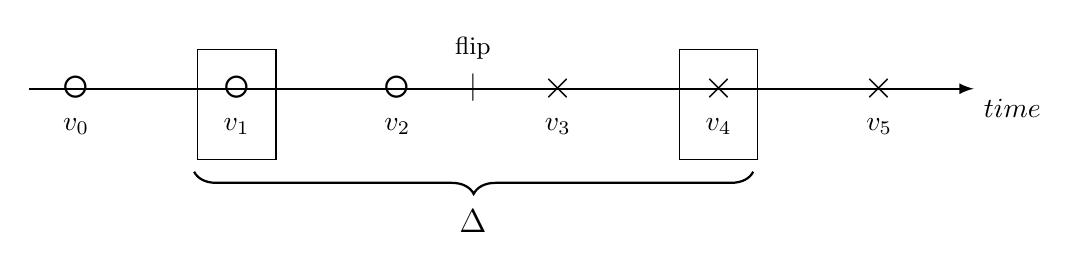
\begin{tikzpicture}[scale=1, line/.style={>=latex}] 

	\coordinate (t0) at (0, 0);
	\coordinate (t1) at (12, 0);

	\coordinate (b0) at (2.1, 0);
	\coordinate (b1) at (9.2, 0);

	\draw[->, line, color=black, thick]
		(t0) --
			node [pos=0.05, below=-8.5pt] {\huge $\circ$}
			node [pos=0.05, below=7pt] {$v_0$}
			node [pos=0.22, below=-8.5pt] {\huge $\circ$}
			node [pos=0.22, below=7pt] {$v_1$}
			node [pos=0.39, below=-8.5pt] {\huge $\circ$}
			node [pos=0.39, below=7pt] {$v_2$}
			node [pos=0.47, below=-9pt] {$ \mathbf{|} $}
			node [pos=0.47, above=7pt] {\small flip}
			node [pos=0.47, below=40pt] {\large $\Delta$}
			node [pos=0.56] {\Large $\times$}
			node [pos=0.56, below=7pt] {$v_3$}
			node [pos=0.73] {\Large $\times$}
			node [pos=0.73, below=7pt] {$v_4$}
			node [pos=0.90] {\Large $\times$}
			node [pos=0.90, below=7pt] {$v_5$}
			node [at end, below right] {$time$}
		(t1);

	\draw[draw=black] (2.14,0.5) rectangle ++ (1,-1.4);
	\draw[draw=black] (8.26,0.5) rectangle ++ (1,-1.4);
	
	\draw [
	    thick,
	    decoration={
		brace,
		amplitude=8pt,
		mirror,
		raise=30pt
	    },
	    decorate
	] (b0) -- (b1);

\end{tikzpicture}


